% !TEX TS-program = xelatex
% !TEX encoding = UTF-8 Unicode

\documentclass[AutoFakeBold]{LZUThesis}
\usepackage{wasysym}
\usepackage{enumitem}
\usepackage[most]{tcolorbox}
\usepackage{multirow}
\usepackage{tikz}
\usetikzlibrary{arrows.meta, decorations.markings}
\usepackage{hyperref}
\usepackage[numbers,sort&compress]{natbib}
\newcommand{\upcite}[1]{\textsuperscript{\textsuperscript{\cite{#1}}}}
\allowdisplaybreaks[4]

\begin{document}

\title{{实验一数据运算:定点加法}}

\entitle{Experiment 1 Data Calculation: Fixed-point Addition}

\author{生物信息学班 李泽华 320210928501}
\major{计算机组成原理}
\advisor{高平}
\college{生命科学学院}
\grade{2021级}


\frontmatter

% \ZhAbstract{
% }{
% }

%\EnAbstract{
%}{
%}

\customcontent

\mainmatter

% \chapter{\texorpdfstring{绪 \quad 论}{绪论}}
\chapter{实验目的}
\begin{enumerate}
    \item 熟悉 LS-CPU-EXB-002 实验箱和软件平台。
    \item 掌握利用该实验箱各项功能开发组成原理和体系结构实验的方法。
    \item 理解并掌握加法器的原理和设计。
    \item 熟悉并运用 verilog 语言进行电路设计。
    \item 为后续设计 CPU 的实验打下基础。
\end{enumerate}
\chapter{实验背景}
\section{数据的表示}
    \subsection{原码}
    原码, 是电脑运算的名词,是指“未经更改”的码。为了便于ALU的设计,又发展出反码、补码等转换过的码。\par
    原码是指一个二进制数左边加上符号位后所得到的码,且当二进制数大于0时,符号位为0;二进制数小于0时,符号位为1;二进制数等于0时,符号位可以为0或1(+0/-0)。\par
    \subsection{补码}
    补码, 是一种用二进制表示有符号数的方法,也是一种将数字的正负号变号的方式,常在计算机科学中使用。补码以有符号比特的二进制数定义。\par
    正数和0的补码就是该数字本身再补上最高比特0。负数的补码则是将其绝对值按位取反再加1。par
    补码系统的最大优点是可以在加法或减法处理中,不需因为数字的正负而使用不同的计算方式。只要一种加法电路就可以处理各种有号数加法,而且减法可以用一个数加上另一个数的补码来表示,因此只要有加法电路及补码电路即可完成各种有号数加法及减法,在电路设计上相当方便。\par
    补码系统的0就只有一个表示方式,这和反码系统不同(在反码系统中,0有二种表示方式),因此在判断数字是否为0时,只要比较一次即可。\par
    \begin{table}[htbp]
        \centering
        \caption{原码、反码、补码}
        \begin{tabular}{cccc|cccc}
            \hline
            数字 & 原码 & 反码 & 补码 & 数字 & 原码 & 反码 & 补码 \\
            \hline
            0 & 0000 & 0000 & 0000 & -1 & 1001 & 1110 & 1111 \\
            \hline
            1 & 0001 & 0001 & 0001 & -2 & 1010 & 1101 & 1110 \\
            \hline
            2 & 0010 & 0010 & 0010 & -3 & 1011 & 1100 & 1101 \\
            \hline
            3 & 0011 & 0011 & 0011 & -4 & 1100 & 1011 & 1100 \\
            \hline
        \end{tabular}
    \end{table}

\section{定点加法}
由于计算机中定点数均以补码的方式表示和存储,采用补码表示法进行加减运算比原码方便多了,因为不论是正还是负,机器总是做加法,减法运算可变成加法运算。\par
二进制加法规则为: 0+0=0, 0+1=1, 1+0=1, 1+1=0(进位1)。\par
\subsection{一位全加器}
由真值表得:
\begin{equation}
    \begin{aligned}
        S & = A \oplus B \oplus C_{in} \\
        C_{out} & = (A \land B) \lor (C_{in} \land (A \oplus B))
    \end{aligned}
\end{equation}

\subsection{RCA}
可以使用多个一位全加器来构成N位加法器,其中对应低位的全加器将其进位输出信号Cout连接到高一位的全加器的进入输入端Cin。这种构成多位加法器的形式被称为“波纹进位加法器”或“脉动进位加法器”(ripple-carry adder),“波纹”形象地描述了进位信号依次向前传递的情形。

波纹进位加法器的电路布局形式较为简单,设计这种电路花费时间较短。然而,波纹进位加法器的进位输出、输入所经过的路径上比其他布局方式具有较多的逻辑门,高位的计算必须等待低位的进位输出信号被计算出来才能开始,因此造成了更大的延迟时间。

\subsection{CLA}
CLA(Carry Look Ahead)超前进位加法器是一种通过预先计算进位信号的加法器,它通过预先计算进位信号来减少延迟时间。CLA加法器的基本思想是将进位信号的计算从低位向高位推进,使得高位的进位信号不再依赖于低位的进位信号,从而减少了延迟时间。

原理: 
令$G_i = A_i \land B_i, P_i = A_i \oplus B_i$,则公式(1)可改写为:
\begin{equation}
    \begin{aligned}
        G_i & = A_i \land B_i \\
        P_i & = A_i \oplus B_i \\
        C_{i+1} & = G_i \lor (P_i \land C_i)
    \end{aligned}
\end{equation}

\subsection{加法溢出}
加法溢出是指两个正数相加得到负数,或者两个负数相加得到正数的情况。

可以使用Cs Xor Cp 来判断是否溢出,其中Cs为最高位的进位输出,Cp为最高位的进位输入。即:
\begin{equation}
    OV = Cs \oplus Cp
\end{equation}


\chapter{实验任务与要求}
\begin{enumerate}
    \item 阅读 LS-CPU-EXB-002 实验箱相关文档,熟悉硬件平台,特别需要掌握利用显示屏观察特定信号的方法。学习软件平台和设计流程。
    \item 熟悉计算机中加法器的原理。
    \item 自行设计本次实验的方案,画出结构框图,详细标出输入输出端口,本次实验的加法器可以使用全加器自己搭建加法模块,也可以在 verilog 中直接使用“+”(系统是自动调用库里加法 IP,且面积时序更优),依据教师要求选择一种方法实现。
    \item 根据设计的实验方案,使用 verilog 编写相应代码。
    \item 对编写的代码进行仿真,得到正确的波形图。
    \item 将以上设计作为一个单独的模块,设计一个外围模块去调用该模块,见图
    \item 将编写的代码进行综合布局布线,并下载到实验箱中的 FPGA 板上进行演示。
\end{enumerate}
\section{实验要求}
\begin{enumerate}
    \item 做好预习:\par
        1) 了解软硬件平台;\par
        2) 掌握定点加法的工作原理;\par
        3) 确定定点加法的输入输出端口设计;\par
        4) 在课前画好设计框图或实验原理图;\par
        5) 如果对 FPGA 板了解的话,可确定设计中与 FPGA 板上交互的接口,画出包含外围模块的整体设计框图,即补充完善图 2.1。\par
    \item 实验实施:\par
        1) 确认定点加法的设计框图的正确性;\par
        2) 编写 verilog 代码;\par
        3) 对该模块进行仿真,得出正确的波形,截图作为实验报告结果一项的材料;\par
        4) 完成调用定点加法模块的外围模块的设计,并编写代码;\par
        5) 对代码进行综合布局布线下载到实验箱里 FPGA 板上,进行上板验证。\par
    \item 实验检查:\par
        1) 完成上板验证后,让指导老师或助教进行检查,进行现场演示,可对演示结果进行拍照作为实验报告结果一项的材料。\par
    \item 实验报告的撰写:\par
        1) 实验结束后,需按照规定的格式完成实验报告的撰写。\par
\end{enumerate}

\chapter{实验结果}
\section{32位串行加法器}
    \subsection{设计思想}
    先设计一个简单的一位全加器模块, 用32个全加器, 前一个的cout与下一个的cin相连, 组成一个32位的串行加法器。
    \subsection{一比特全加器}
    %verilog代码
    \lstset{language=verilog}
    \begin{lstlisting}
module bit_adder(
    input   Bit_1, Bit_2,
    input   Cin,
    output  So,
    output  Co);

    wire Xor;

    assign Xor = Bit_1 ^ Bit_2;
    assign So = Xor ^ Cin;
    assign Co = Xor & Cin | Bit_1 & Bit_2;
endmodule
    \end{lstlisting}

% 插入图片
    \begin{figure}[htbp]
        \centering
        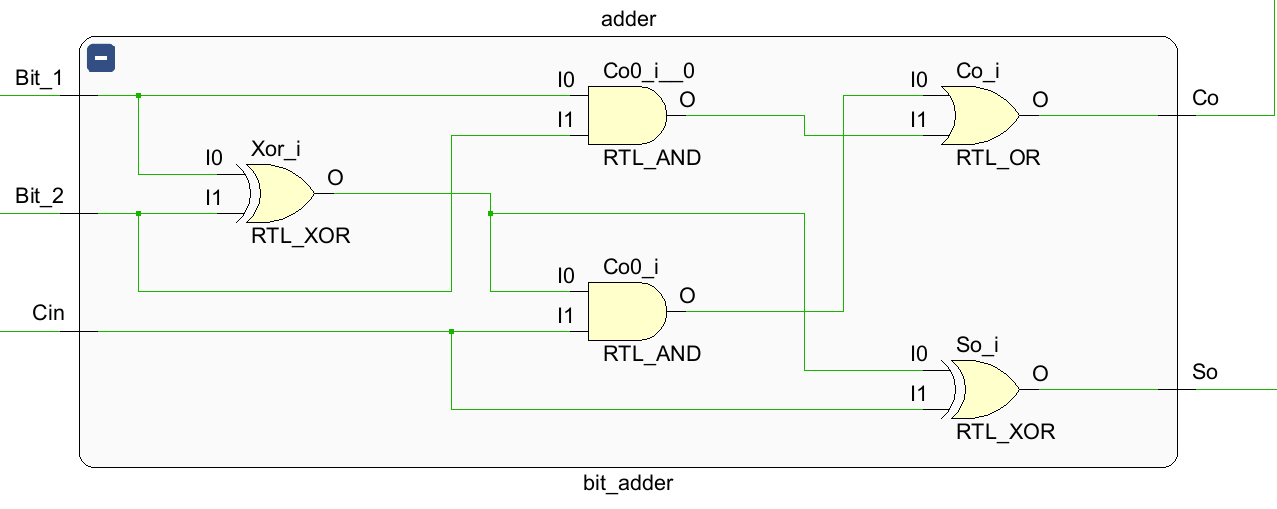
\includegraphics[width=0.8\textwidth]{./img/bitadder}
        \caption{上述代码组成的一位全加器}
    \end{figure}
    \subsection{32位串行加法器}
    \begin{lstlisting}
module full_adder1(
    input [31:0] Num_1, Num_2,
    input        Cin,
    output [31:0] Sum,
    output        Cout,
    output        OV, // overflow
    output        ZF, // zero flag
    output        NF, // negative flag
    output        CF  // carry flag
);

    genvar i;
    wire [31:0] Cout_wire;

    generate
        bit_adder adder(
            .Bit_1(Num_1[0]),
            .Bit_2(Num_2[0]),
            .Cin(Cin),
            .So(Sum[0]),
            .Co(Cout_wire[0])
        );
        for (i = 1; i < 32; i = i + 1)
        begin
            bit_adder adder(
                .Bit_1(Num_1[i]),
                .Bit_2(Num_2[i]),
                .Cin(Cout_wire[i - 1]),
                .So(Sum[i]),
                .Co(Cout_wire[i])
            );
        end
    endgenerate

    assign Cout = Cout_wire[31];
    assign OV = Cout_wire[30] ^ Cout_wire[31];
    assign ZF = Sum == 0;
    assign NF = Sum[31];
    assign CF = Cout_wire[31];

endmodule
    \end{lstlisting}
    \begin{figure}[htbp]
        \centering
        \subfloat[]{
            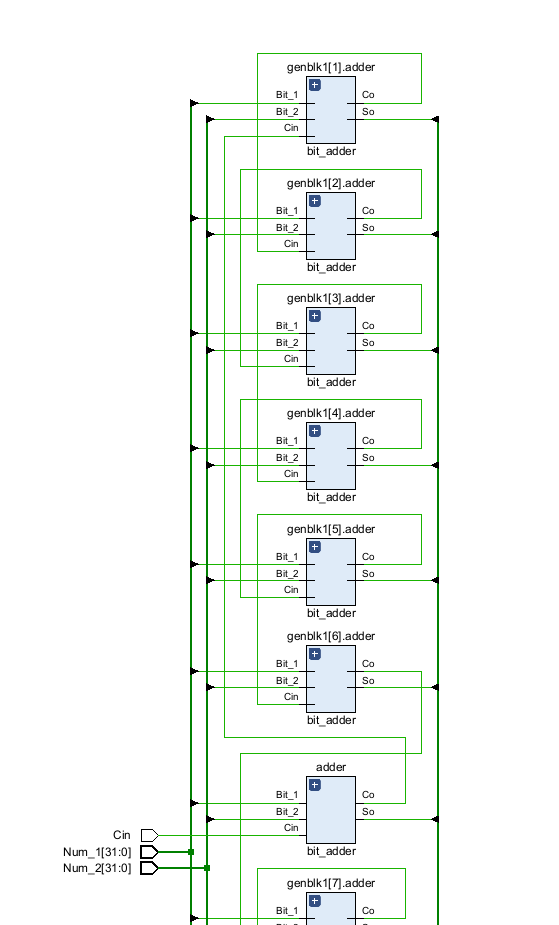
\includegraphics[width=0.3\textwidth]{./img/32bitadder}
        }
        \centering
        \subfloat[]{
            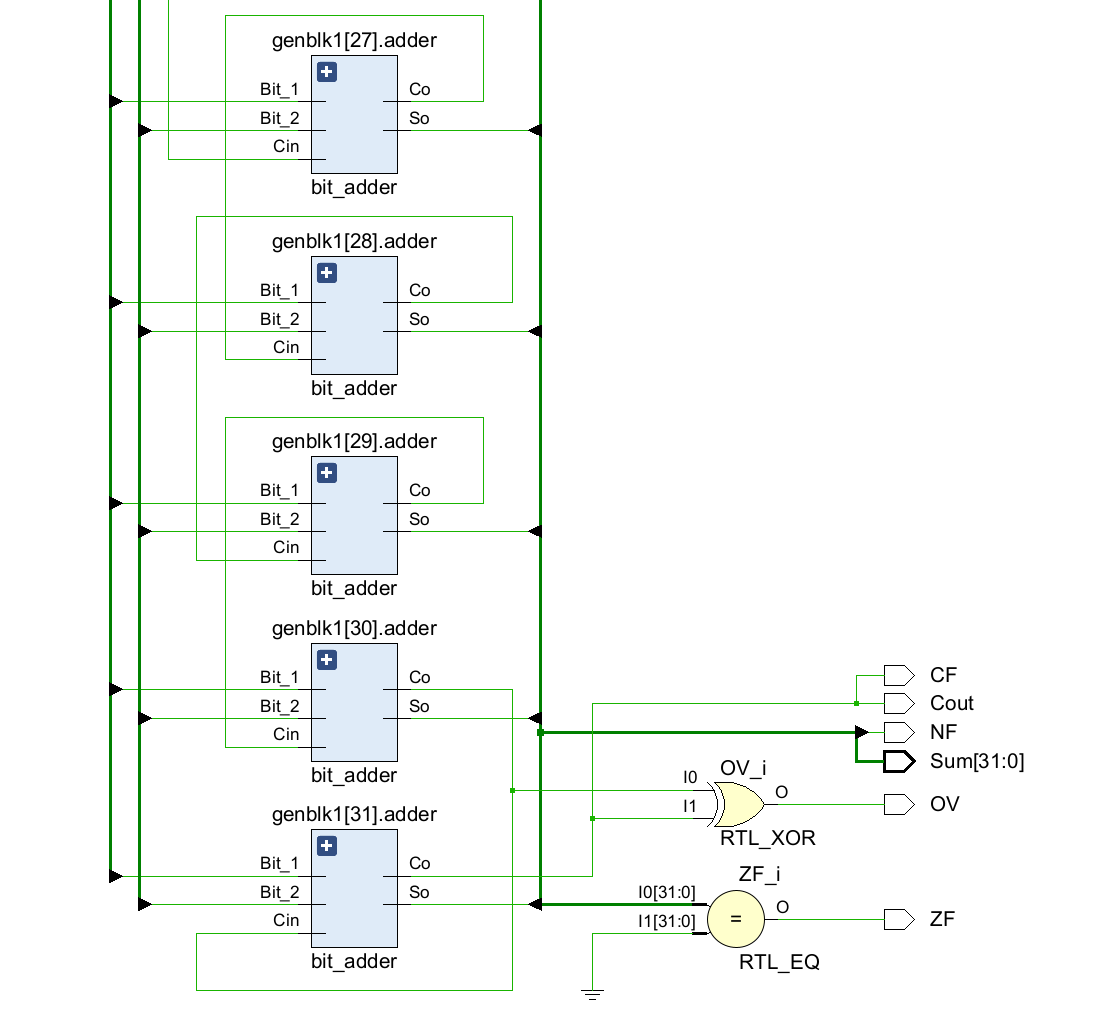
\includegraphics[width=0.3\textwidth]{./img/32bitadder2}
        }
        \caption{32位串行加法器}
    \end{figure}
\subsection{测试数据与仿真结果}
    \begin{lstlisting}
module test ;
    // input 
    reg [31:0] operand1, operand2;
    reg        carry_in;
    
    // output
    wire [31:0] sum;
    wire        carry_out;
    wire       overflow;
    wire       zero_flag;
    wire       negative_flag;
    wire       carry_flag;


    full_adder1 u_adder(
        .Num_1   (operand1),
        .Num_2   (operand2),
        .Cin     (carry_in),
        .Sum     (sum),
        .Cout    (carry_out),
        .OV      (overflow),
        .ZF      (zero_flag),
        .NF      (negative_flag),
        .CF      (carry_flag)
    );

    initial begin 
        operand1 = 0;
        operand2 = 0;
        carry_in = 0;
        #100;

        operand1 = 1;
        operand2 = 2;
        carry_in = 1;
        #100;

        operand1 = 32'h80000000;
        operand2 = 32'hffffff00;
        carry_in = 0;
        #100;
    end
endmodule
    \end{lstlisting}
    \begin{figure}[htbp]
        \centering
        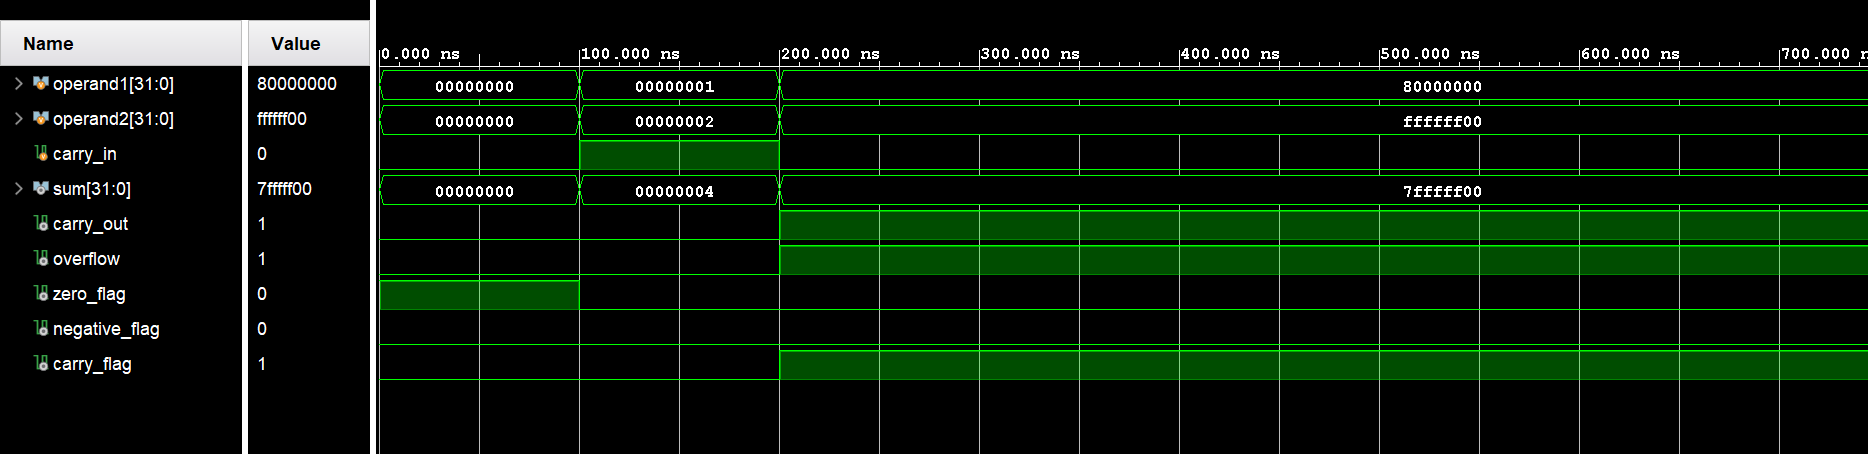
\includegraphics[width=0.8\textwidth]{./img/32bitadder_simulate}
        \caption{32位串行加法器仿真结果}
        \label{fig:32bitadder_simulate}
    \end{figure}
\section{16位并行加法器}
\subsection{设计思想}
    和高平老师讨论后我了解到前面的加法器是一个串行的加法器, 速度比较慢, 经过查阅书本, 我认为超前进位加法器是一个更好的选择.\par
    基本的设计思路是: 先使用超前进位加法器设计一个4位的并行加法器, 再将4个4位的并行加法器串联, 组成一个16位的并行加法器。
\subsection{4位并行加法器}
    \begin{lstlisting}
module one_bit_adder( // 改造的一位全加器
    input Bit_1, Bit_2,
    input Cin,
    output So,
    output G, P
    );

    assign G = Bit_1 & Bit_2;
    assign P = Bit_1 ^ Bit_2;
    assign So = Cin ^ P;
endmodule

module four_bit_CG(  // 4位进位生成器
    input [3:0] p, g,
    input cin,
    output [4:1] co,
    output po, go
);

assign co[1] = g[0] | p[0] & cin;
assign co[2] = g[1] | p[1] & g[0] | p[1] & p[0] & cin;
assign co[3] = g[2] | p[2] & g[1] | p[2] & p[1] & g[0] | p[2] & p[1] & p[0] & cin;
assign co[4] = g[3] | p[3] & g[2] | p[3] & p[2] & g[1] | p[3] & p[2] & p[1] & g[0] | p[3] & p[2] & p[1] & p[0] & cin;

assign po = p[3] ^ g[3];
assign go = g[3];

endmodule

module four_bit_LCU_adder( // 4位超前进位加法器
    input [3:0] input_1, input_2,
    input cin,
    output [3:0] sum,
    output go,
	output po,
    output co
);

wire [3:0] p, g;
wire [4:1] c;
//wire po, go;

four_bit_CG four_bit_CG_1(
    .p(p),
    .g(g),
    .cin(cin),
    .co(c),
    .po(po),
    .go(go)
);

one_bit_adder bit_adder_1(
    .Bit_1(input_1[0]),
    .Bit_2(input_2[0]),
    .Cin(cin),
    .So(sum[0]),
    .P(p[0]),
    .G(g[0])
);

one_bit_adder bit_adder_2(
    .Bit_1(input_1[1]),
    .Bit_2(input_2[1]),
    .Cin(c[1]),
    .So(sum[1]),
    .P(p[1]),
    .G(g[1])
);

one_bit_adder bit_adder_3(
    .Bit_1(input_1[2]),
    .Bit_2(input_2[2]),
    .Cin(c[2]),
    .So(sum[2]),
    .P(p[2]),
    .G(g[2])
);

one_bit_adder bit_adder_4(
    .Bit_1(input_1[3]),
    .Bit_2(input_2[3]),
    .Cin(c[3]),
    .So(sum[3]),
    .P(p[3]),
    .G(g[3])
);

assign co = c[4];
endmodule
    \end{lstlisting}
    \begin{figure}[htbp]
        \centering
        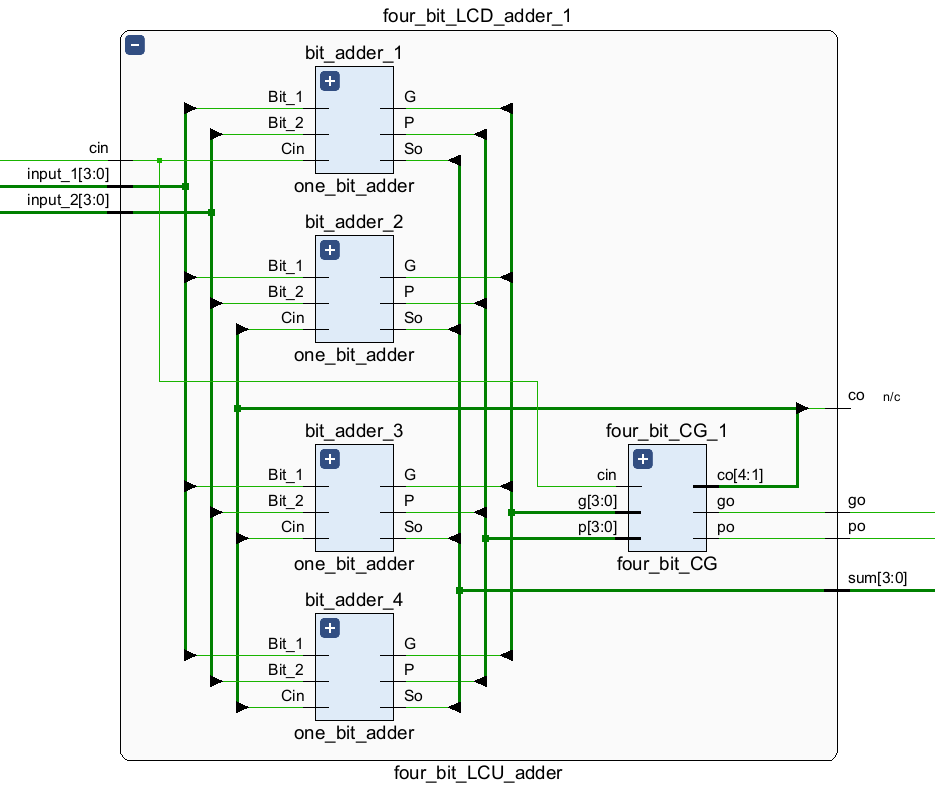
\includegraphics[width=0.8\textwidth]{./img/4bitadder}
        \caption{4位并行加法器}
    \end{figure}

\subsection{16位并行加法器}
    \begin{lstlisting}
module sixteen_bit_full_adder(
    input [15:0] Num_1, Num_2,
    input Cin,
    output [15:0] Sum,
    output go, po,
    output Cout,
    output OV, // overflow
    output ZF, // zero flag
    output NF, // negative flag
    output CF  // carry flag
);

wire [3:0] G, P, C;

four_bit_ALU four_bit_ALU_1(
    .p(P),
    .g(G),
    .cin(Cin),
    .co(C),
    .po(po),
    .go(go)
);

four_bit_LCU_adder four_bit_LCD_adder_1(
    .input_1(Num_1[3:0]),
    .input_2(Num_2[3:0]),
    .cin(Cin),
    .sum(Sum[3:0]),
    .go(G[0]),
    .po(P[0])
);

four_bit_LCU_adder four_bit_LCD_adder_2(
    .input_1(Num_1[7:4]),
    .input_2(Num_2[7:4]),
    .cin(G[0]),
    .sum(Sum[7:4]),
    .go(G[1]),
    .po(P[1])
);

four_bit_LCU_adder four_bit_LCD_adder_3(
    .input_1(Num_1[11:8]),
    .input_2(Num_2[11:8]),
    .cin(G[1]),
    .sum(Sum[11:8]),
    .go(G[2]),
    .po(P[2])
);

four_bit_LCU_adder four_bit_LCD_adder_4(
    .input_1(Num_1[15:12]),
    .input_2(Num_2[15:12]),
    .cin(G[2]),
    .sum(Sum[15:12]),
    .go(G[3]),
    .po(P[3])
);

assign Cout = C[3];
assign OV = C[3] ^ C[2];
assign ZF = Sum == 0;
assign NF = Sum[15];
assign CF = C[3];

endmodule
    \end{lstlisting}

    \begin{figure}[htbp]
        \centering
        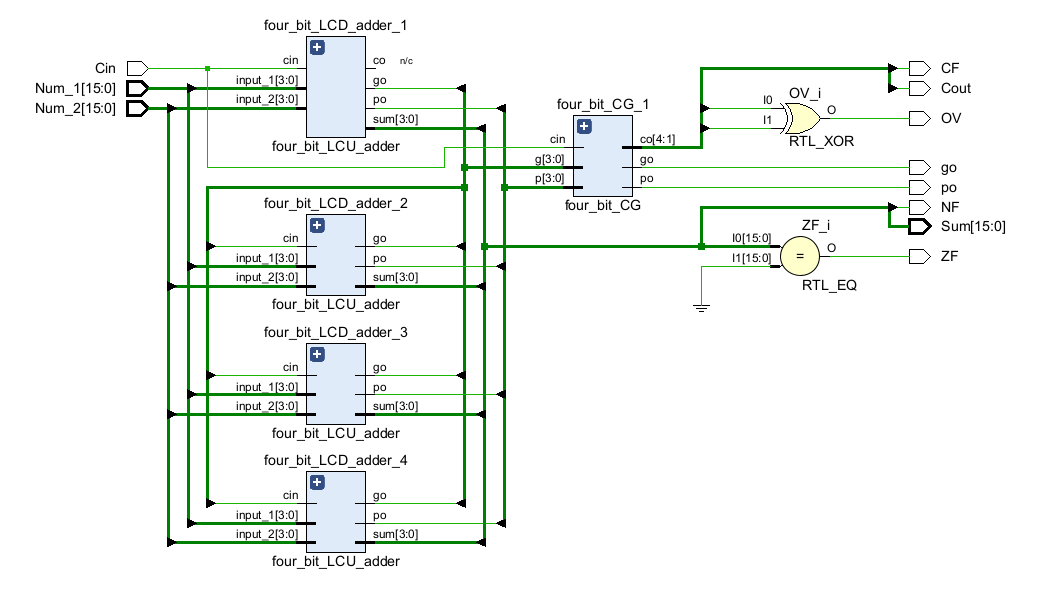
\includegraphics[width=0.8\textwidth]{./img/16bitadder}
        \caption{16位并行加法器}
    \end{figure}

\subsection{测试数据与仿真结果}
    \begin{lstlisting}
module test ;
    // input 
    reg [15:0] operand1, operand2;
    reg        carry_in;
    
    // output
    wire [15:0] sum;
    wire       carry_out;
    wire       g;
    wire       p;
    wire       overflow;
    wire       zero_flag;
    wire       negative_flag;
    wire       carry_flag;

    sixteen_bit_full_adder sixteen_bit_full_adder_1(
        .Num_1(operand1),
        .Num_2(operand2),
        .Cin(carry_in),
        .Sum(sum),
        .Cout(carry_out),
        .po(p),
        .go(g),
        .OV(overflow),
        .ZF(zero_flag),
        .NF(negative_flag),
        .CF(carry_flag)
    );

    initial begin 
        operand1 = 0;
        operand2 = 0;
        carry_in = 0;
        #100;

        operand1 = 1;
        operand2 = 2;
        carry_in = 1;
        #100;

        operand1 = -1;
        operand2 = -2;
        carry_in = 0;
        #100;

        operand1 = 1000_0000_0000_0000;
        operand2 = 1000_0000_0000_0000;
        carry_in = 0;
    end
endmodule

    \end{lstlisting}

    \begin{figure}[htbp]
        \centering
        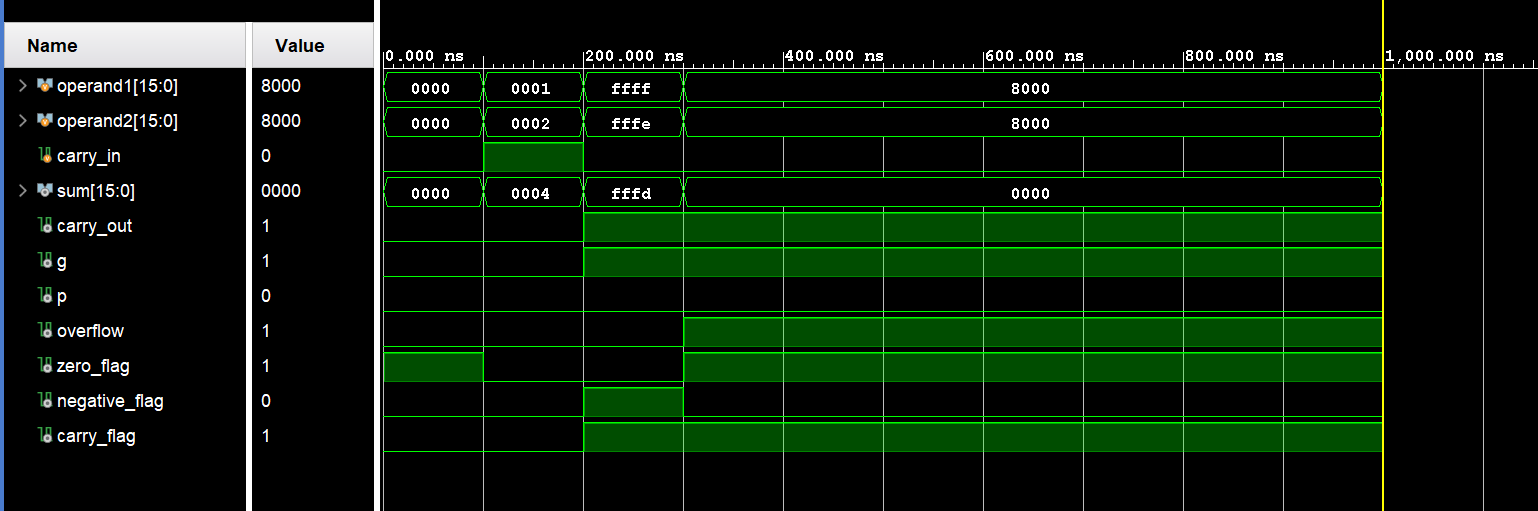
\includegraphics[width=0.8\textwidth]{./img/16bitadder_simulate}
        \caption{16位并行加法器仿真结果}
        \label{fig:16bitadder_simulate}
    \end{figure}




\section{原反码转换}

添加如下代码, 实现原反码转换:
    \begin{lstlisting}
module complement(
    input [15:0] Num,
    output reg [15:0] Comp
);

always @* begin
    //Comp = Num[15] ? ~Num + 1 : Num;
    if (Num[15] == 1) begin
        Comp[14:0] = ~Num[14:0];
        Comp[15] = 1;
        Comp = Comp + 1;
    end
    else begin
        Comp = Num;
    end
end

endmodule
    \end{lstlisting}
在16位加法器前后实例化该模块, 实现原反码转换, 结果如下:

    \begin{figure}[htbp]
        \centering
        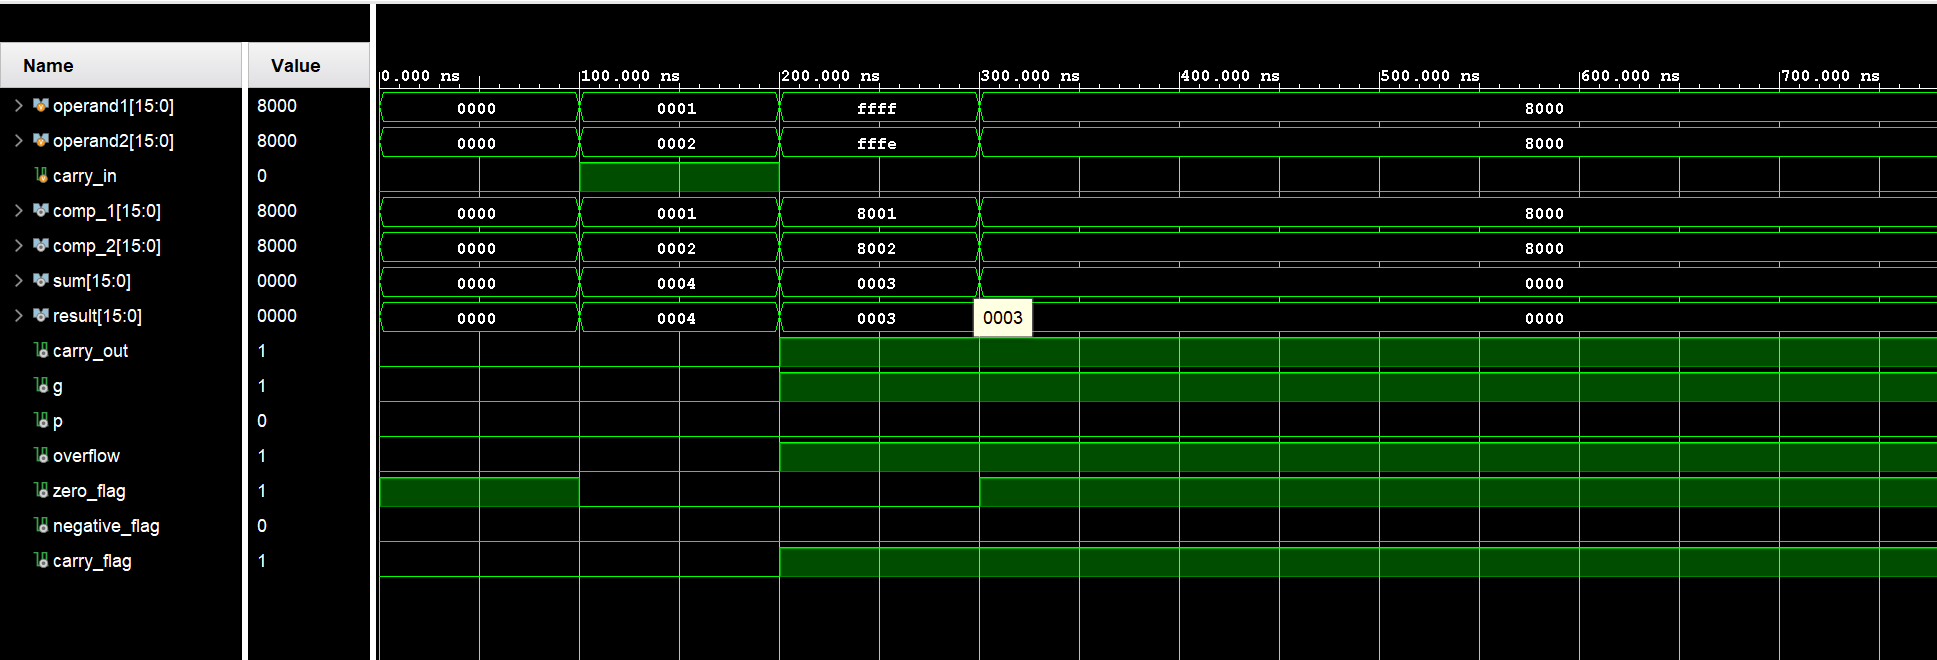
\includegraphics[width=0.8\textwidth]{./img/16bitadderwithcomplement}
        \caption{带有原反码转换的16位并行加法器运行结果}
        \label{fig:16bitadderwithcomplement}
    \end{figure}

\chapter{思考与讨论}
\section{课后问题}
\begin{enumerate}
    \item 答: 不论是有符号还是无符号数, 都会自动转化为补码进行运算. 
    如图\ref{fig:16bitadder_simulate}所示, 在第三次运算中, -1转换为ffff, -2转换为fffe, cin为0, 结果fffd为-3, 与预期结果一致.
    \item IP库使用补码进行运算
    \item 4种标志位分别为: OV(溢出), ZF(零标志), NF(负数标志), CF(进位标志), 
    溢出通过Cs Xor Cp判断, 进位通过最高位的进位输出信号判断, 零标志通过判断结果是否为0判断, 负数标志通过最高位判断.
    具体实现如代码所示.
    \item 如图\ref{fig:16bitadderwithcomplement}所示, 第二次运算由于输入为正数, 原码与补码相同. 
    第三次输入的-1被自动转换为补码ffff后又被转换了一次变为原码8001, operand -2同理, 最终被转化为8002, 进入加法器进行运算后得到了0003, 发生溢出且答案错误.
    因此这里不应该手动进行原反码转换.
\end{enumerate}
\section{讨论}
自己实现的32位串行加法器和16位并行加法器, 而不是简单的调用IP库, 我对加法器的原理有了更深的理解, 课本上学到的原理看似简单, 但在具体实现的时候总是会遇到各种问题, 
通过查阅各种资料并与老师讨论, 我很开心我最终能够成功.

在这一过程中我对verilog这门语言也有了一些简单的了解, 对verilog所谓的并行有了自己的一点理解. 
在我看来, verilog与我之前学的任何一种语言都不一样, 相反, 我觉得他和tikz有一些相似之处. 
这样说是因为我认为verilog所谓的并行编程实际上是在用编程语言绘制电路图, 就像使用tikz绘图一样,
然后运行这一电路图, 由于在运行中, 所有并行的电路会被同时接入, 产生了并行的效果, 不知道这样的理解是否正确.

当然我认为我的本次实验中也有很多不足之处, 比如我对verilog的理解还不够深入, 代码的风格也不够规范, 代码的复用性也不够好, 有很多地方可以改进.
也由于知识的欠缺, 我并不能准确的计算出加法器的延时.
%论文后部
\backmatter


%=======%
%引入参考文献文件
%=======%
%\bibdatabase{bib/database}%bib文件名称 仅修改bib/ 后部分
%\printbib
%\nocite{*} %显示数据库中有的,但是正文没有引用的文献



\Appendix

%\Thanks


%\Grade %这一句才是成绩页,上面是填写


\end{document}
